% !TeX root = RJwrapper.tex
\title{Image Analysis with R: a Review}
\author{Stefan R\"{o}diger, Hinrich Winther and Micha\l{} Burdukiewicz}

\maketitle

%An abstract of less than 150 words.
\abstract{
Management, display, and processing of biological and medical imaging data is 
an important task in life sciences and medical research. R is a powerful 
cross-platform, which can handle most task statistical computing tasks in 
the same environment. The aim of this mini-review is to give a brief overview 
about image processing software for the R statistical computing environment. 
When it comes to image analysis, R may appear to provide only few tools on the 
first sight. However, a systematic analysis of the existing packages shows 
shows that a huge potential for numerous applications.
}

\section{Introduction}

\begin{itemize}
\item Digital image processing?
\item Where is it used?
\end{itemize}

There are numerous software tools that have been made available for digital 
image aquisition and processing \citep{wiesmann_review_2015, chieco_image_2013}. 
The scientific background of the useres is deliberately broad. This includes 
biologists, biostatisticians, physicians and others, who fundamentally make use 
of the similar image analysis techniques. From discussion with peers we learned 
that knowledge of image processing is gained by self-study. In particular, 
learning of several programming languages may hamper the scientist to focus on 
their scientific aim. R \citep{R} is \textit{de facto} the \textit{lingua 
franca} of statistical bioinformatics and therefore used in numerous research 
disciplines \citep{rodiger_r_2015}. It is a powerful tool for statistical data 
analysis. It comes to no surprise that software packages for digital image 
processing have been implemented \citep{frery_introduction_2013}. In this 
review, we give a current overview of the R ecosystem about which software 
packages exist and which deficits they may expose in comparison to other 
software packages. We aimed to aggregate information about R packages available 
on CRAN, Bioconductor \citep{gentleman_bioconductor:_2004}, RForge or github.

Analysis of 2D and 3D digital images is a bridge technology which has been used 
to unravel quantitative and qualitative gene expression data (mRNA and protein 
level), cellular interactions and diagnostic data. In particular, 
immunoflourescence images were analyzed in relation to cell structures, tissues 
and organs \citep{chieco_image_2013, rodiger_highly_2013, 
schierack_species-specific_2014, willitzki_new_2012}.

We performed two image processing case studies were we applied selected 
packages for immunoflourescence image analysis and RMI data. 

There are numerous software packages for the analysis of image data 
\citep{wiesmann_review_2015}. However, R is quite functional when it comes to 
digital image analysis.

image processing capabilities of Cell-ID and data analysis by the statistical 
programming framework R for quantifying various cellular features (e.g., volume, 
total and subcellular fluorescence localization) from sets of microscope 
images of individual cells \citep{bush_using_2012}


\section{Give me a title}

General image processing and analysis


\citep{tabelow_modeling_2012, tabelow_dti:_2014}

Murrel \citep{murrell_raster_2011}
\CRANpkg{mmand} \citep{clayden_mmand:_2016}

CRAN provides well established packages. These are \CRANpkg{jpeg}, \CRANpkg{png} 
and \CRANpkg{tiff} to read, write and display bitmap JPEG, PNG and TIFF images. 
The development of the \CRANpkg{ripa} \citep{perciano_ripa:_2014} package was 
started in 2005 by Talita Perciano. This package can be used to processes and 
analyses RGB, LAN (multispectral) and AVIRIS (hyperspectral) images. Recent 
advances of \CRANpkg{ripa} make it a promising tool for analysis of large 
datasets. The vast amount of image data is becoming more and more and essential 
part of Big Data analysis pipelines. R is among the frequently used for data 
mining and analysis. It comes to no surprise the commercial and non-commercial 
entities make heavy use of R \citep{chen_big_2014}. \BIOpkg{EBImage} 
\citep{pau_ebimager_2010} is presumably the most comprehensive package and the 
foundation for many other R packages in the context of microscopy-based cellular 
assays \citep{gowen_near_2015}. This package offers tools to transform (e.g, 
rotate) the images, segment object (e.g., cells) and extract quantitative 
descriptors. The early version of \BIOpkg{EBImage} used the Magick++ interface 
to the ImageMagick image processing library \citep{sklyar_image_2006}.

\section{General image processing and analysis}

This section may contain a figure such as Figure~\ref{figure:bead}.

\begin{figure}[htbp]
  \centering
  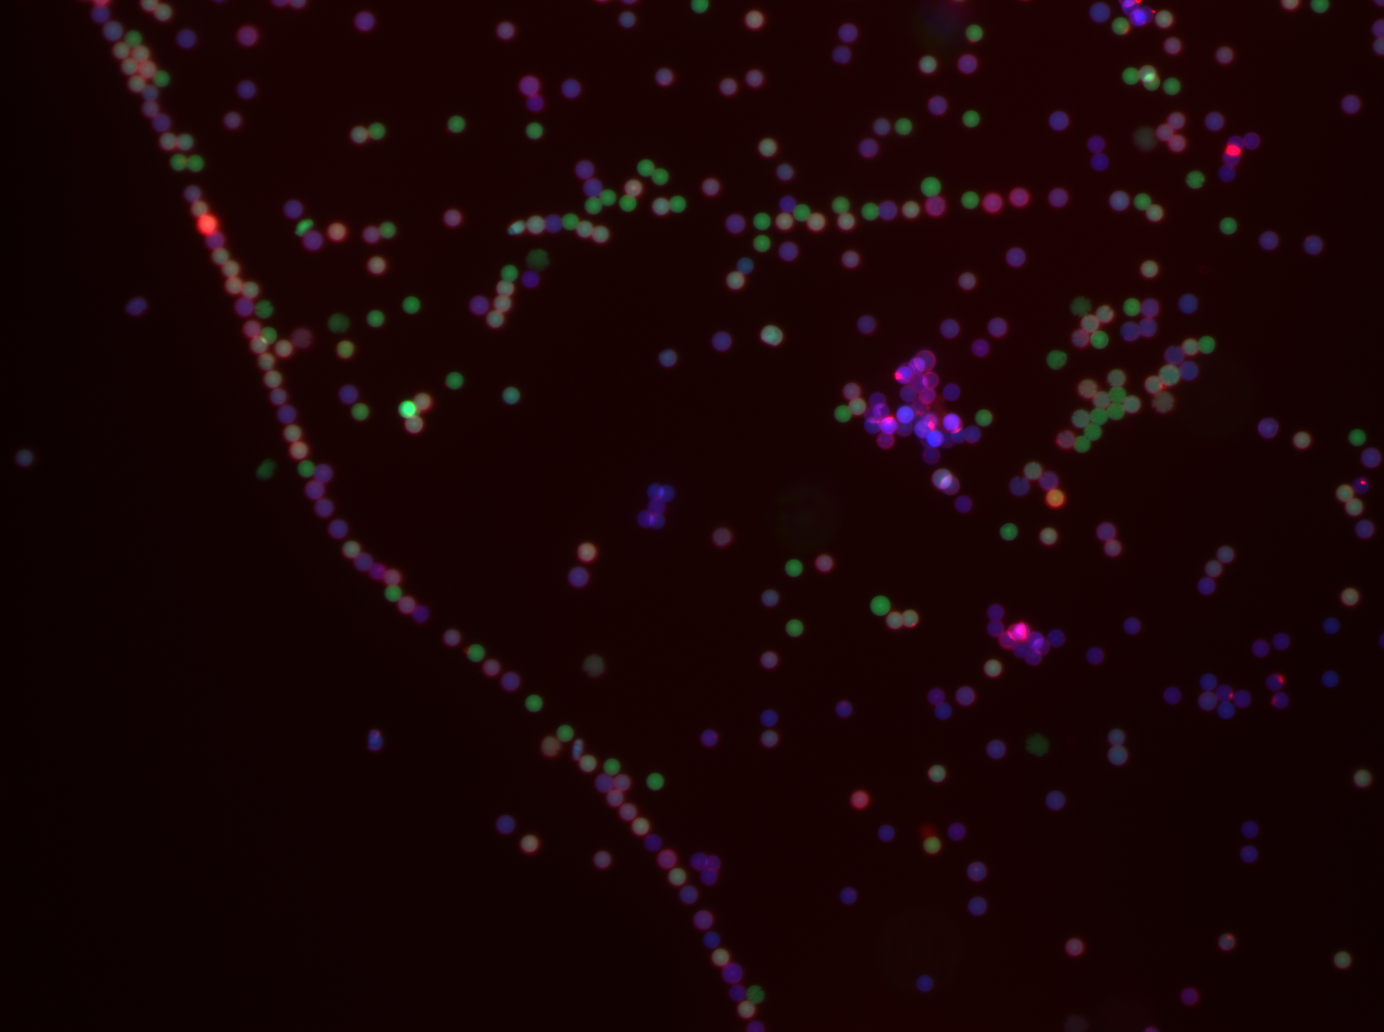
\includegraphics[clip=true,trim=0.1cm 0.3cm 0.2cm 0.1cm, width=12cm]{bead}
  \caption{The logo of R.}
  \label{figure:bead}
\end{figure}

\section{segmentation}

\citep{holmes_interactive_2009}

\CRANpkg{adimpro} is a package for manipulation of digital images and the 
Propagation Separation approach for smoothing digital images \citep{polzehl_adaptive_2007}.
For example, image analysis is used for the detection and quantification of 
cell patterns and array technologies like microarrays and bead-based assays 
\citep{rodiger_highly_2013, willitzki_new_2012, willitzki_fully_2013, 
dunning_beadarray:_2006}.
Several software packages have been developed. imageJ belongs to the most 
used and cited tools. When it comes to R numerous packages exist, which can 
be readily integrated in the analysis routines \citep{frery_introduction_2013}.

The accuracy of image segmentation is a critical step in a computer-aided 
diagnosis systems. The recognition of mitotic cells and the classification of 
fluorescent patterns is heavily dependent on this. Immunofluorescent images 
of cell, such as Hep-2, exhibit a high variability due a wide range of staining 
patterns and intensity levels (FIGURES OF CELLS), the presence of mitotic 
cells and  artifacts. The later may be caused by uneven illumination and 
photo-bleaching effects \citep{tonti_automated_2015}.

Intensity inhomogeneity (bias field) is a common artefact in 
magnetic resonance (MR) images, which hinders successful automatic segmentation. \citep{ivanovska_efficient_2016}


\begin{example}
  x <- 1:10
  result <- myFunction(x)
\end{example}


\section{Applications}

\section{Examples}
\subsection{Statistical analysis of functional magnetic resonance imaging data}

Statistical analysis of functional magnetic resonance imaging (fMRI) data  is a non-invasive neuroimaging technique.

largely used in clinical routine and advanced brain research

\CRANpkg{AnalyzeFMRI} \citep{marchini_analyzefmri:_2002, bordier_temporal_2011} and \CRANpkg{fmri} 
\citep{polzehl_fmri:_2007} and are packages for the analysis of Magnetic 
Resonance Imaging (MRI) and functional Magnetic Resonance Imaging (fMRI) data, 
respectively.

Eventually these de 

Others include \CRANpkg{dcemriS4} \citep{dunning_beadarray:_2006, frery_introduction_2013}.

\subsection{Analysis of fluorescence image data}

\CRANpkg{CRImage} package \citep{failmezger_crimage:_2012} for tumor image analysis


\subsection{Analysis of microbead assays}

\citep{rodiger_nucleic_2014, rodiger_highly_2013}

\begin{example}
# Detailed installation instructions are available at 
# http://bioconductor.org/packages/EBImage/

# Install the EBImage from Bioconductor
source("http://bioconductor.org/biocLite.R")
biocLite("EBImage")

# Load the EBImage package
require(EBImage)


\end{example}


\section{Graphical User Interface for Digital Image Analysis}

There exist also R graphical user interfaces \citep{rodiger_rkward:_2012} which 
can be used for for image processing. Bio7 is an integrated development 
environment based on the Eclipse Rich Client Platform (RCP). The main purpose of 
this tool is the modeling and analysis of ecological systems. However, Bio7 is 
not restricted to this discipline. T he application contains GUIs and plugins 
for simulation and analysis tasks. Interestingly, one of these plugins is an 
adaption image application ImageJ and another is available for a bidirectional 
Java connection to R. This means that data can be transferred from and to ImageJ 
and R.

\section{Performance}

Micha\l{}, would you like to take this section?


Requirements for recent research include the rapid processing of massive amounts 
of image data (Mega to Tera byte scale) that modern technologies (e.g., 
microscopes, MRI scanner) produce nowadays. Preferably, affordable personal desktop
computers should be usable. R has several disadvantages when it comes to memory management
and GPU and CPU usage ...

\section{Summary}

Many scientist are using R. However, it appears that only few make use of the 
image analysis tools currently available. We would like to raise awareness for 
the fact that R provides sophisticated packages for digital image analysis. The 
central advantage is that all analysis is conducted within the same environment 
accross most  platforms. Added values for the user are that there is less need 
to learn a new programming languages and that all analysis can be performed in a 
consistent and cross-platform environment. Table~\ref{table:packages} gives an 
overview of R packages currently available. We found that functions from the 
packages can be easily combinded to conduct manipulations and analysis (object 
transformations, measurements, object counting, grey level statisitcs, 
binarization, etc) at advanced levels. The organization of such functions in 
coustumized packages is straigthforward even for more complex analysis 
functions.

\citep{rodiger_intestinal_2015} or combined assays of microbeads and cells \citep{scholz_second_2015, grossmann_simultaneous_2016}

While evaluation the packages we ended up with experiences regarding the 
installation and maintenance. Bascially all installation were well instructed. 
For example, the installation of sophisticated packages like \BIOpkg{EBImage} is 
well documented. However, many packages depend on a number of third-party 
packages. This applies also to \CRANpkg{EBImage} which requires tiff and 
fftwtools.

Others and we recommend to make use of packages for reproducible research 
\citep{rodiger_r_2015}. 

There exist sevel GUI technologies for R which make it possible to integrate 
R code into an easy to master point-and-click interface.


\begin{table}
\begin{center}
\begin{tabular}[c]{llll}
Package & Main function & Comment & Source\\
\CRANpkg{adimpro} & × & × & ×\\
\CRANpkg{AnalyzeFMRI} & × & × & ×\\
\CRANpkg{CRImage} & × & × & Bioconductor\\
\CRANpkg{dcemriS4} & × & × & CRAN\\
\BIOpkg{EBImage} & fancy stuff & well maintained & Bioconductor\\
\CRANpkg{jpeg} & × & × & CRAN\\
\CRANpkg{png} & × & × & CRAN\\
\CRANpkg{ripa} & × & × & ×\\
\CRANpkg{tiff} & × & × & CRAN\\
\emph{videoTools} & video and image analysis & - & RForge\\
\end{tabular}
\end{center}
\caption{\label{table:packages}
R packages. \emph{videoTools}: http://www.rforge.net/videoTools/files/.
}
\end{table}

\bibliography{roediger-winther-burdukiewicz}

\address{Stefan R\"odiger (corresponding author)\\
  orcid.org/0000-0002-1441-6512\\
  Faculty of Natural Sciences\\
  Brandenburg University of Technology Cottbus--Senftenberg\\
  Senftenberg\\
  Germany\\
}
\email{Stefan.Roediger@b-tu.de}

\address{Hinrich Winther\\
  Affiliation\\
  Address\\
  Country\\}
\email{author@work}

\address{Micha\l{} Burdukiewicz\\
  University of Wroclaw\\
  Faculty of Biotechnoloy\\
  Department of Genomics\\
  Wroclaw\\
  Poland}
\email{michalburdukiewicz@gmail.com}
